\documentclass[11pt]{article}
\usepackage[margin=1in]{geometry}
\usepackage[T1]{fontenc}
\usepackage{lmodern}
\usepackage{microtype}
\usepackage{amsmath,amssymb,amsthm}
\usepackage{graphicx}
\usepackage[hidelinks]{hyperref}

\newtheorem{theorem}{Theorem}
\newtheorem{lemma}{Lemma}
\newcommand{\B}{\mathcal B}
\newcommand{\Trc}{\mathcal B^1}
\newcommand{\QS}{Q_{\!S}}
\newcommand{\QH}{Q_{\!H}}

\title{Heisenberg quantum channels are operator-norm closed\\
\large A full answer to the closure question in arXiv:2012.03496}
\author{Run \texttt{fa\_banach\_001}, lane 1 (GPT5.6)}
\date{11 August 2026}

\begin{document}
\maketitle

\noindent\fbox{\parbox{0.94\textwidth}{\textbf{Status: candidate full result,
likely valid.} For separable complex Hilbert spaces $\mathcal G,\mathcal H$,
the set $\QH(\mathcal G,\mathcal H)$ is closed in
$\B(\B(\mathcal G),\B(\mathcal H))$ for the operator norm.}}

\section{Source and exact question}

Vom Ende's thesis \cite{vomEnde} defines a Schr\"odinger quantum channel as a
completely positive trace-preserving map
\[
 T:\Trc(\mathcal H)\longrightarrow \Trc(\mathcal G)
\]
and a Heisenberg quantum channel as an ultraweakly continuous completely
positive unital map
\[
 S:\B(\mathcal G)\longrightarrow \B(\mathcal H).
\]
Their respective sets are denoted $\QS(\mathcal H,\mathcal G)$ and
$\QH(\mathcal G,\mathcal H)$.

Immediately after Proposition 2.3.13, the source asks whether
$\QH(\mathcal G,\mathcal H)$ is closed in the \emph{full} bounded-map space
$\B(\B(\mathcal G),\B(\mathcal H))$ \cite[p.~48]{vomEnde}. The exact source
passage is reproduced in Figure~\ref{fig:question}.

\begin{figure}[ht]
\centering

\includegraphics[width=\textwidth]{figures/open_problem_crop.png}
\caption{The operator-norm closure question, arXiv:2012.03496v2, printed
page 48 (physical PDF page 62).}
\label{fig:question}
\end{figure}

\section{Proof intuition}

The source already identifies the two channel pictures by an isometric
bijection: take the Banach-space adjoint. It also proves that the
Schr\"odinger channel set is operator-norm closed, hence complete. An
isometry preserves Cauchy sequences and limits, so its image---the entire
Heisenberg channel set---is complete in the ambient operator norm. Complete
subsets of metric spaces are closed. The weak-star continuity concern raised
after the question never enters, because the norm-isometric preadjoint
correspondence constructs the limiting normal map directly.

\section{Formal proof}

\begin{lemma}\label{lem:image}
Let $X$ be a complete metric space, $Y$ a metric space, and
$J:X\to Y$ an isometry. Then $J(X)$ is closed in $Y$.
\end{lemma}

\begin{proof}
If $J(x_n)\to y$ in $Y$, then $(J(x_n))$ is Cauchy. Isometry makes $(x_n)$
Cauchy, hence $x_n\to x$ for some $x\in X$. Again by isometry,
$J(x_n)\to J(x)$, and uniqueness of metric limits gives $y=J(x)$.
\end{proof}

\begin{theorem}\label{thm:closure}
Let $\mathcal G,\mathcal H$ be separable complex Hilbert spaces. Then
\[
 \QH(\mathcal G,\mathcal H)
 \quad\text{is operator-norm closed in}\quad
 \B\bigl(\B(\mathcal G),\B(\mathcal H)\bigr).
\]
\end{theorem}

\begin{proof}
The source's Corollary 2.3.12 says that every
$S\in\QH(\mathcal G,\mathcal H)$ has the form $S=T^*$ for a unique
$T\in\QS(\mathcal H,\mathcal G)$. The paragraph preceding Proposition
2.3.13, together with its footnote 33, says that
\[
 J:\QS(\mathcal H,\mathcal G)\longrightarrow
 \QH(\mathcal G,\mathcal H),\qquad J(T)=T^*,
\]
is a surjective isometry for the operator norms \cite[pp.~46--47]{vomEnde}.

Proposition 2.3.13(i) states that $\QS(\mathcal H,\mathcal G)$ is
operator-norm closed in
\[
 \B\bigl(\Trc(\mathcal H),\Trc(\mathcal G)\bigr)
\]
\cite[p.~47]{vomEnde}. Consequently
$\QS(\mathcal H,\mathcal G)$ is complete. Lemma~\ref{lem:image}, applied to
the displayed isometry with codomain the full space
$\B(\B(\mathcal G),\B(\mathcal H))$, shows that its image is closed there.
Surjectivity identifies that image with $\QH(\mathcal G,\mathcal H)$.
\end{proof}

The two decisive source inputs are shown together in
Figure~\ref{fig:inputs}.

\begin{figure}[ht]
\centering
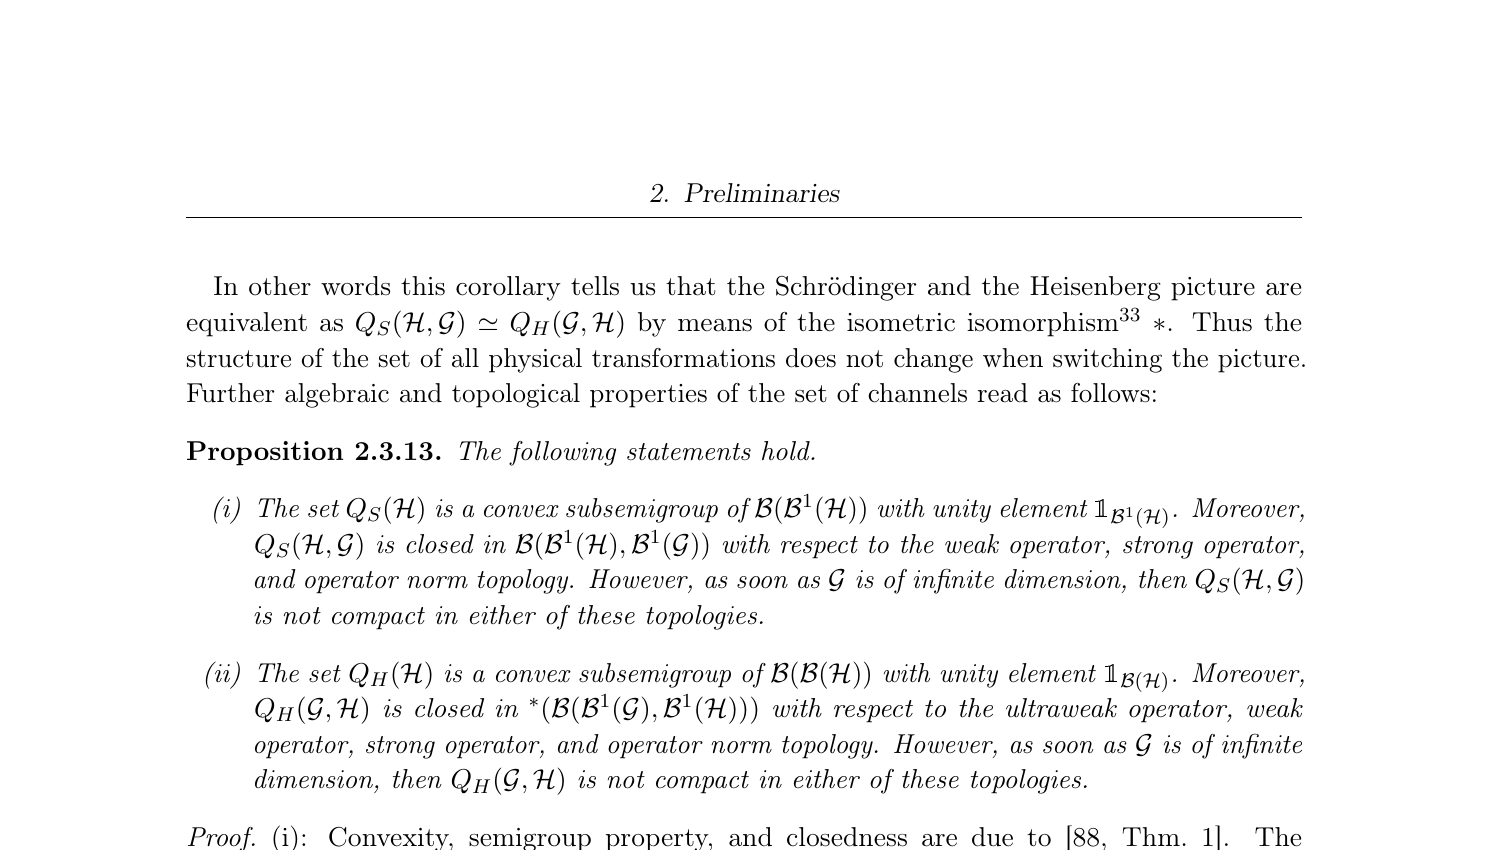
\includegraphics[width=\textwidth]{figures/source_duality_closedness_crop.png}
\caption{The source states both the isometric Schr\"odinger--Heisenberg
identification and operator-norm closedness of $\QS$ (printed page 47).}
\label{fig:inputs}
\end{figure}

\section{Independent sequence audit}

For clarity, suppose $S_n\in\QH(\mathcal G,\mathcal H)$ and
$\lVert S_n-S\rVert\to0$ in the full mapping space. Write $S_n=T_n^*$ using
Corollary 2.3.12. Then
\[
 \lVert T_n-T_m\rVert=\lVert T_n^*-T_m^*\rVert
 =\lVert S_n-S_m\rVert,
\]
so $T_n$ converges in operator norm to some $T$. Proposition 2.3.13(i) gives
$T\in\QS$. Moreover $T_n^*\to T^*$ in norm, while $T_n^*=S_n\to S$.
Thus $S=T^*\in\QH$. This repeats the completeness proof without hiding any
topological interface.

\section{Verification, limitations, and novelty}

The proof uses only three statements explicitly present on adjacent source
pages: surjectivity of the adjoint correspondence, its norm-isometry, and
norm-closedness of $\QS$. No finite-dimensional approximation, compactness,
or weak-star limit argument is used. Hence the source's warning that weaker
operator topologies may fail to preserve weak-star continuity does not affect
the theorem.

The claim is restricted to operator-norm closure and to the source's separable
Hilbert-space setting. It does not assert compactness or closure for weaker
topologies.

On 11 August 2026, exact searches of the run registry and the solution,
attempt, and proof-gap indexes found no packet for arXiv:2012.03496. Bounded
primary-arXiv searches used the exact closure sentence, ``Heisenberg quantum
channels operator norm closed,'' and ``normal unital completely positive maps
norm closed.'' They found the source and later quantum-control work, but no
paper explicitly recording this corollary. Novelty confidence is moderate:
the argument appears unrecorded, but it is an immediate overlooked consequence
of the source's own adjacent results.

Human review should verify that the norm in footnote 33 is the ambient
operator norm and that Corollary 2.3.12 is onto the full $\QH$ appearing in
the question. Both are explicit in the reproduced source pages.

\begin{thebibliography}{1}
\bibitem{vomEnde}
F. vom Ende,
\emph{Reachability in Controlled Markovian Quantum Systems: An
Operator-Theoretic Approach}, arXiv:2012.03496v2, 2020.
\end{thebibliography}

\end{document}
